% !TEX encoding = UTF-8 Unicode

\Chapter{Tesztek, eredmények bemutatása}
Azokat a szűrőket amelyeket a \textbf{4. fejezet}ben tárgyaltam, nem csak képek átalakítására használtam, hanem videókon is teszteltem. Ebben a fejezetben szeretném leírni ezzel kapcsolatban a tapasztalataimat. 
\\

\noindent Először a technikai adatait szeretném leírni a számítógépnek amin írtam és futtattam a programokat. Ez egy MacBook Pro  2014 mid, 2.6 GHz Intel Core i5 processzorral, 8 gb memóriával, Intel Iris 1536 MB grafikus kártyával és macOS High Sierra operációs rendszerrel.
\Section{Szűrők tesztelése képeken}
Először képeken teszteltem a szűrőimet, azokon a képeken amiket más a \textbf{3. fejezetben} bemutattam. Az első tesztekben azt mutatom meg, hogy mennyi milliszekundum alatt készül el a kép és melyik művelet mennyi ideig tart, természetesen milliszekundumban mutatom meg aztokat is.\\\\
\textbf{Cartoon-style filter}\\\\
Ennél a filternél a teljes képfeldolgozási idő: 89,485 ms\\
amiből,\\
Kép betöltés: 4,714 ms\\
Gauss piramisban a kép kicsinyítése: 1.153 ms\\
A kétoldalú szűrő: 21,757 ms\\
Gauss piramisban a kép nagyitása normál méretre: 1,467 ms\\
A kép konvertálása színesből szürkernyalatossá valamint a medián szűrés: 8,902 ms\\
Az adaptív küszöbölés: 0,837 ms\\
A bitwise\_and függvény: 0,525 ms
\newpage
\begin{figure}[ht]
\centering
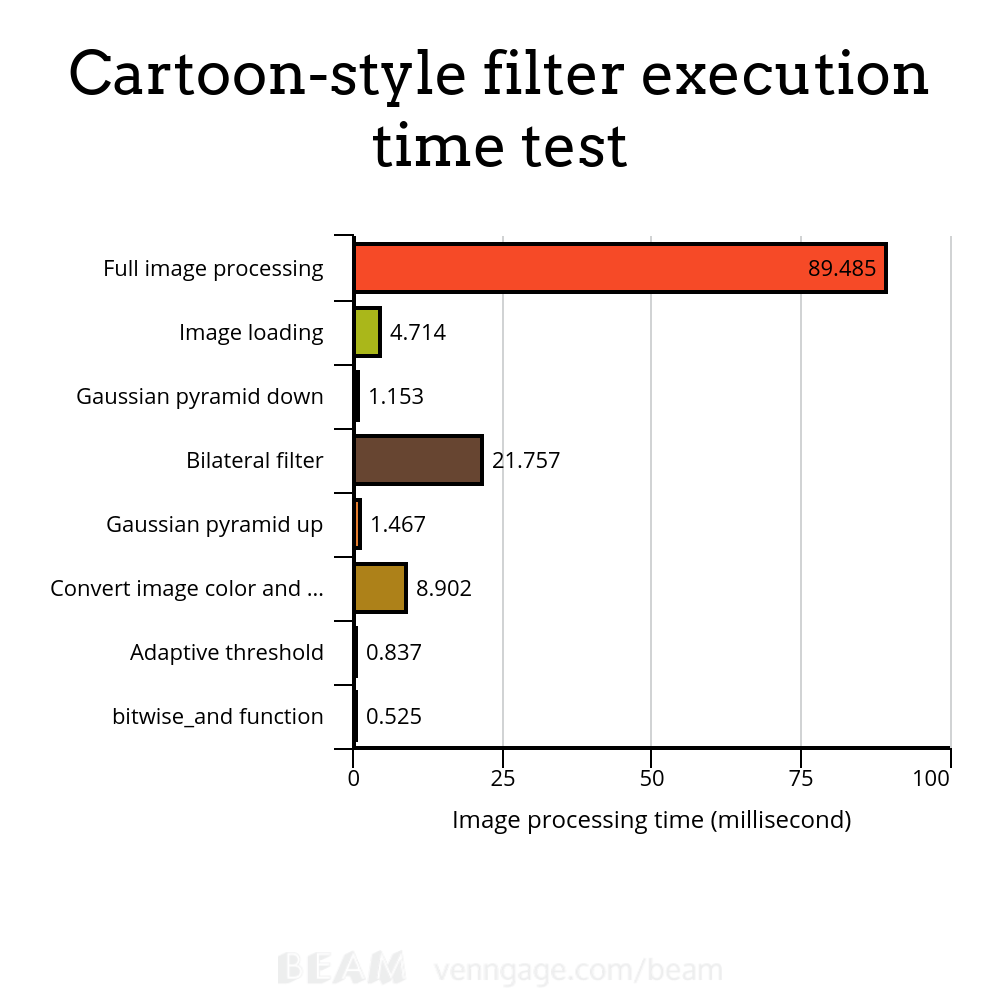
\epsfig{file=kepek/cartoon_style_test.png,scale=0.3}
\caption{Grafikonon ábrázolva a Cartoon-style filter feldolgozási ideje} 
\label{fig: graf1}
\end{figure}
\noindent Látható, hogy ha össze adjuk külön külön a függvények feldolgozási idejét akkor, $4,714+1,153+21,757+1,467+8,902+0,837+0,525=39.355$ ms-t kapunk, ami nem egyezik meg a 89,485 ms-os teljes kép feldolgozással. Ez a különbség annak tudható be, hogy még néhány művelet például, néhány deklarálás nincs benne, valamint azok a függvények sem amivel magát a teszteket végeztem és azok kiíratásuk, ha külön külön nézzük a függvényeket. \\ \\
%grafikon-https://beam.venngage.com
\textbf{Pencil sketch filter}\\\\
Ennél a filternél a teljes képfeldolgozási idő: 70,016 ms\\
amiből,\\
Kép betöltés: 9,737 ms\\
Medián szűrő: 1,417 ms\\
Gauss szűrő: 7,863 ms\\
Gauss szűrő és a medián szűrő elosztása: 0,436 ms\\
Kontraszt széthúzás : 0,147 ms\\
Az adaptív küszöbölés: 1,944 ms\\\\
\begin{figure}[ht]
\centering
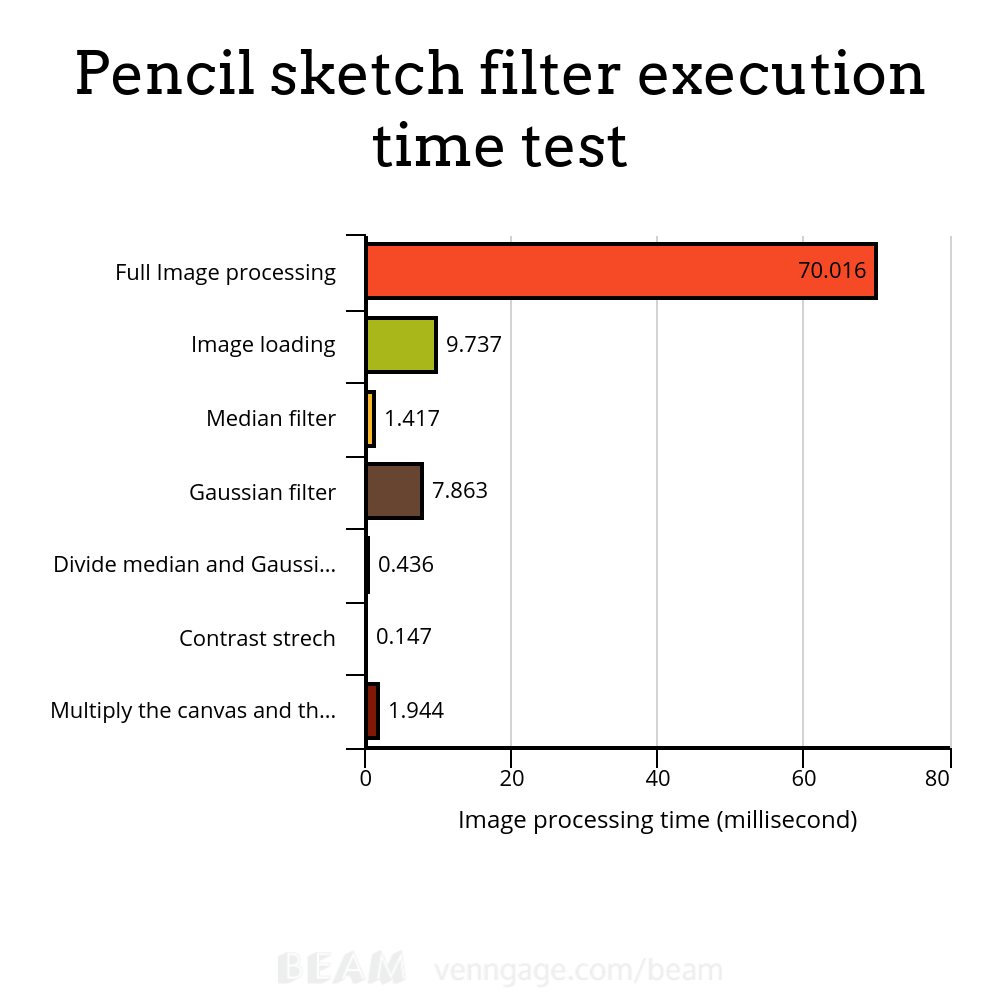
\epsfig{file=kepek/pencil_sketch_test.png,scale=0.3}
\caption{Grafikonon ábrázolva a Pencil sketch filter feldolgozási ideje} 
\label{fig: graf2}
\end{figure}
\noindent Itt is látható, hogy ha össze adjuk külön külön a függvények feldolgozási idejét akkor, $9,737+1,417+7,863+0,436+0,147+1,944=21.544$ ms-t kapunk, ami nem egyezik meg a 70,016 ms-os teljes kép feldolgozással. \\ \\
%grafikon-https://beam.venngage.com
\textbf{Cartoon filter}\\\\
Ennél a filternél a teljes képfeldolgozási idő: 66,614 ms\\
amiből,\\
Kép betöltés: 4,937 ms\\
Medián szűrő: 9,892 ms\\
Laplace éldetektálás: 1,193 ms\\
Küszöbölés: 0,436 ms\\
Kontraszt széthúzás : 0,371 ms\\
Maszk másolása a képre: 0,987 ms\\\\
\begin{figure}[ht]
\centering
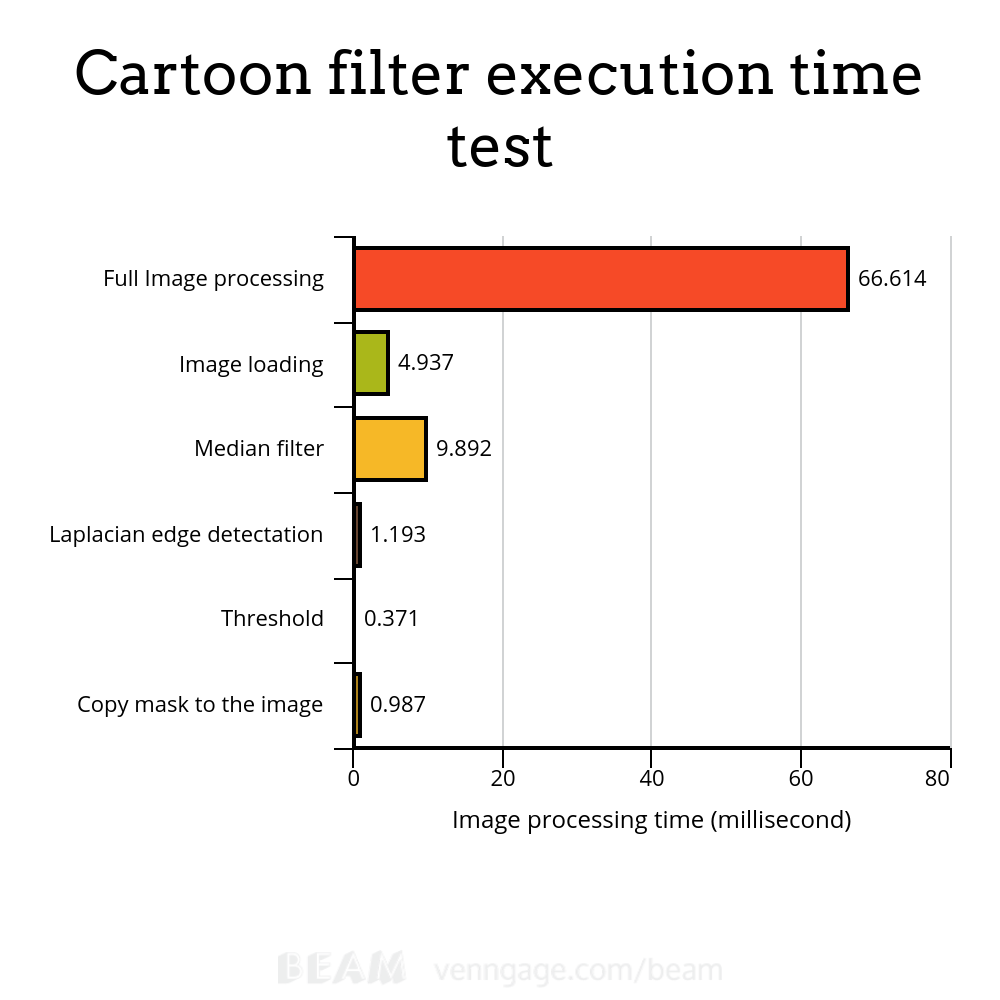
\epsfig{file=kepek/cartoon_test.png,scale=0.24}
\caption{Grafikonon ábrázolva a Cartoon  filter feldolgozási ideje} 
\label{fig: graf3}
\end{figure}
\noindent Itt is látható, hogy ha össze adjuk külön külön a függvények feldolgozási idejét akkor, $4,937+9,892+7,863+0,436+0,371+0,987=24,486$ ms-t kapunk, ami nem egyezik meg a 66,614 ms-os teljes kép feldolgozással. \\ \\
%grafikon-https://beam.venngage.com
\newpage
\textbf{Aquarelle-style filter}\\
Ennél a filternél a teljes képfeldolgozási idő: 524,863 ms\\
amiből,\\
Kép betöltés: 6,476 ms\\
Medián szűrő: 0,88 ms\\
Maszk másolása a képre: 467,275 ms\\\\
\begin{figure}[ht]
\centering
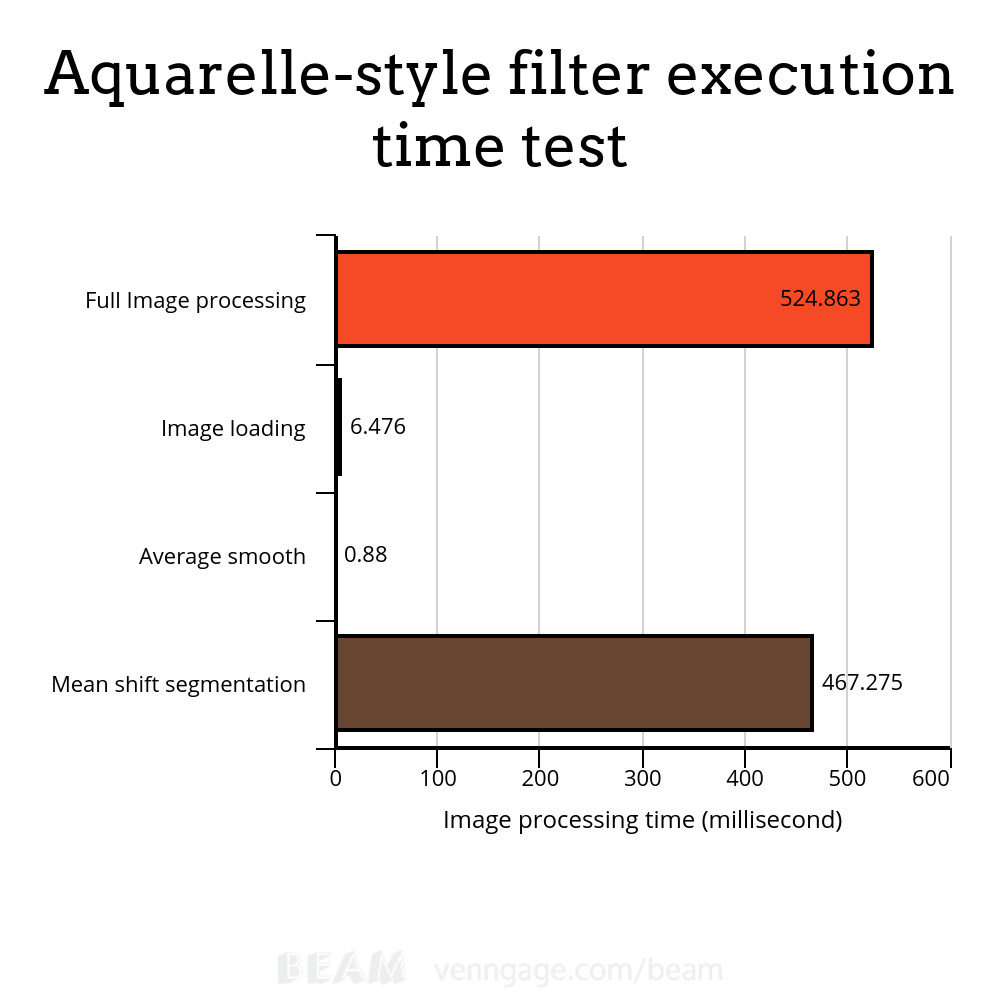
\epsfig{file=kepek/aquarelle_style_test.png,scale=0.24}
\caption{Grafikonon ábrázolva a Aquarelle-style filter feldolgozási ideje} 
\label{fig: graf4}
\end{figure}
\noindent Itt is látható, hogy ha össze adjuk külön külön a függvények feldolgozási idejét akkor, $6,476+0,88+467,275=474.631$ ms-t kapunk, ami nem egyezik meg a 524,863 ms-os teljes kép feldolgozással.
%grafikon-https://beam.venngage.com
\Section{Szűrők tesztelése videókon és valós időben}




%4-6 oldal
